%Linea Para poder completar automaticamente las citas con el Sublime
%No hace el documento, se puede borrar esta linea si no se usa el Sublime
%------------------------------------------------------------------------------
 \newcommand{\NoBiblioMicro}[1]{
 \ifthenelse{\equal{#1}{verdadero}}{}{\bibliography{Referencias/base_bibliografica}}
 \NoBiblioMicro{verdadero}}
 %-----------------------------------------------------------------------------

%Formato (Nombre de capitulo largo o corto), nombre del capitulo, resumen y estilo de la
%Portada del Capitulo
%------------------------------------------------------------------------------
 
 %Formato en si, titulo en dos renglones
 \FormatoCapituloDosLineas
 
 %Nombre y etiquete para referir
 \chapter{Microfabricación de los electrodos}
 \label{chap:Microfabricacion}

 %Para que no salga el numero de pagina en la portada del capitulo
 \thispagestyle{empty}
	
 %Resumen del Capitulo en Italica
 \noindent\textit{En este capitulo repasamos los resultados obtenidos en la fabricación de los electrodos. Se analizan los diseños utilizados, los materiales empleados y las caracterizaciones llevadas a cabo; fundamentalmente el desempeño electroquímico\index{electroquimico} de los electrodos y la compatibilidad con las síntesis sol-gel\index{sol-gel} que se emplearon para depositar las películas mesoporosas sobre ellos; síntesis que fueron ampliamente discutidas en los capítulos previos.
 }
 
 
 %Indice de capitulo alineada al borde inferior de la pagina, nueva pagina
 \vfill
 \minitoc
 \newpage
 %-------------------------------------------------------------------------------

\section{Introducción}

	El diseño de los sensores\index{sensor} abarca desde la elección de los materiales, hasta el diseño de las máscara\index{máscara}s para configurar los electrodos. En el capitulo \ref{chap:Mesoporosos}, ya se discutió la elección de los materiales para conformar la película delgada \index{película!delgada}mesoporososa, con la cual se recubren los electrodos para formar el elemento <<activo>> de los sensores.

	Respecto de los electrodos se eligió Au\index{oro} como material para los mismos. Son conocidas las excelentes propiedades de este metal  para llevar a cabo reaccciones de oxido-reducción, lo que lo hace especialmente útil en mediciones electroquímica\index{electroquimico}s\index{electroquimico}.\cite{Wi2000,Pumera2007,Gewirth2004,Villullas2000} Si bien, como acabamos de decir, el Au\index{oro} es el material óptimo para electroquimica, existen otros mas económicos (tintas de carbono, óxido de indio/estaño, carbono vitreo, etc.), sin embargo, su respuesta electroquímica\index{electroquimico} es poco repetible y tienen grandes desviaciones de la idealidad (sobre todo a altas velocidades de barrido). En este trabajo se busca hacer un estudio profundo sobre los mecanismos de transporte\index{transporte} de sonda\index{sonda}s dentro de sistemas porosos, motivo por el cual necesitamos una respuesta electroquimica confiable y repetible.

	%ESCRITO ANTERIORMENTE
		% 	Siempre con la idea de desarrollar un multisensor electroquímico\index{electroquimico}s\index{electroquimico} selectivo, especifico, integrado y escalable decidimos, para logra este fin, explorar las propiedades de las películas delgadas de óxidos mesoporosos descritas con anterioridad. Nos dedicamos, como primera aproximación, a depositar estas películas de óxido sobre otra película delgada, esta vez de Au, que a su vez está depositada sobre algún sustrato\index{sustrato} rígido y térmicamente estable como vidrio\index{vidrio} u silicio, de forma de obtener una estructura bicapa electrodo\textbar mesoporoso. 

		% 	Muchos de los trabajos que figuran el la bibliografía utilizan técnicas de electroquímica\index{electroquimico} como herramienta de caracterización para películas mesoporosas con múltiples propósitos; como inferir estructuras de poros, accesibilidad, deducir propiedades de transporte\index{transporte} y estimar variables del sistema. En este trabajo se plantea el uso de la electroquímica\index{electroquimico}, no solo como herramienta de caracterización de películas mesoporososas sino también como técnica analítica. Para lograr dicho objetivo se evaluó el desempeño electroquímico\index{electroquimico} de los electrodos de Au\index{electrodo!de Au} así como la viabilidad de ser utilizados como sustrato\index{sustrato} para el depósito\index{depósito} de película delgada \index{película!delgada}mesoporosa. Dichas películas serán el elemento activo, que actúa como membrana selectiva de los analitos electroactivos a cuantificar. 

\section{Microfabricación de los sensores}
		
	 	 En las secciones siguientes se discuten los resultados del diseño de los sensores, la fabricación de los electrodos, también se discuten las técnicas de deposito y las caracterizaciones realizadas sobre de los mismos y, por último, su compatibilidad con las técnicas sol-gel\index{sol-gel} para utilizarse como sustratos para las películas mesoporosas funcionales.

  		\subsection{Consideraciones sobre el diseño}

			Desde un principio se surgió la idea de fabricar un sensor\index{sensor} con múltiples electrodos. Los dos diseños de sensores\index{sensor} que se fabricaron en esta tesis tuvieron en cuenta esto, colocando múltiples electrodos por sensor. 

		 \subsubsection{Primer diseño}

		 El primer diseño contempló cuatro electrodos de trabajo\index{electrodo!de trabajo} (ET) por sensor\index{sensor} y preveía utilizar contraeelectrodo (CE) y electrodo de referencia\index{electrodo!de referencia} (ER) externos. 

		 Se trabajó con dimensiones relativamente grandes (los electrodos circulares tienen un radio R=\SI{300}{\um} y los cuadrados el lado de L=\SI{500}{\um}) por dos motivos; 1) ya que fue la primera aproximación para estimar corrientes y, 2) bajar costos en la impresión de máscara\index{máscara}s.
		
				\begin{figure}[th!]
		 	       	\includegraphics[width=\textwidth]{Imagenes/diseno_mascara_v1.pdf}
 		       		\caption[Primer diseño y máscara\index{máscara} de los sensores]{Diseño y máscara\index{máscara} para la primera versión de los electrodos. A) diseño completo con 32 sensores\index{sensor} de 4 ET cada uno, B) Detalles de las marcas de alineación, C) microscopia\index{microscopía} de la máscara\index{máscara} ya impresa donde se ven las imperfecciones de la impresión.}
 		         	\label{fig:diseno_mascara_v1}
 		     		\end{figure}
		
		 La figura \ref{fig:diseno_mascara_v1} muestra este primer diseño donde se puede apreciar que la impresión de la máscara\index{máscara}, no es exactamente igual al diseño, sino que se ve una deformación del mismo dada por la baja resolución de la impresora; estableciendo de esta forma limitaciones en los diseños para usar con con este tipo de máscara\index{máscara}s, la contrapartida es el muy bajo costo de las mismas y la facilidad para obtenerlas en cualquier librería gráfica.
		
 		 \subsubsection{Segundo Diseño}

		 El segundo diseño, mas completo y compacto, está compuesto por sensores\index{sensor} cuadrados de \SI{1}{\cm} de lado. Cada uno tiene, a su vez, 6 ET circulares y dispuestos sobre una circunferencia imaginaria y equiangulares entre ellos. (ver figura \ref{fig:mascara_diseno_v2} y {\ref{fig:diseno_mascara_v1}). Se hicieron 6 sensores\index{sensor} de diámetros variados (con R=\SI{300}{\um},\SI{200}{\um},\SI{150}{\um},\SI{100}{\um} y \SI{20}{\um}), además contempla la integración del CE y del ER en el mismo sensor. El CE se ubica en el centro del diseño y tiene un área 5 veces mayor a la de los ET para no limitar la velocidad de reacción respecto del ET \cite{Wi2000}. El ER se ubica rodeando el CE, dispuestos de esta forma, nos aseguramos que todos los ET se encuentren equidistantes tanto del CE como del ER.

						\begin{figure}[th!]
			 	   	    \begin{subfigure}[t]{0.395\textwidth}
			        	\includegraphics[width=\textwidth]{Imagenes/SistemaA.pdf}
			    		\end{subfigure}
						\begin{subfigure}[t]{0.595\textwidth}
			     		\includegraphics[width=\textwidth]{Imagenes/diseno_3d.jpg}
			        	\end{subfigure}
			     		\caption[Segundo diseño y máscara\index{máscara} de los sensores]{Segundo diseño de los sensores. Izquierda: Diseño de un sensor\index{sensor} con los 6 electrodos de trabajo\index{electrodo!de trabajo}, el contraelectrodo\index{electrodo!contraelectrodo}, el electrodo de referencia\index{electrodo!de referencia} y las marcas de alineación. Derecha: Esquema en perspectiva para un sensor\index{sensor} de \SI{1x1}{\cm} con la celda. En rojo los electrodos y en verde la resina para la celda, el espesor de la misma es de aproximadamente \SI{100}{\um} y puede contener un volumen aproximado de \SI{2}{\ul}.}
			     		\label{fig:mascara_diseno_v2}
			     		\end{figure}

			     			\begin{figure}[th!]
			 	   	    \centering
			 	   	    \begin{subfigure}[t]{0.495\textwidth}
			        	\includegraphics[width=\textwidth]{Imagenes/mascara_revolver_electrodos.pdf}
			       		\caption{Máscara para la segunda versión de los electrodos, la cual contiene 46 sensores\index{sensor} de \SI{1}{cm} de lado cada uno.}
			         	\label{fig:mascara_v2}
			     		\end{subfigure}
			     		\begin{subfigure}[t]{0.495\textwidth}
			     		\includegraphics[width=\textwidth]{Imagenes/impresion_mascaras_V2.pdf}
			    		\caption{Detalle del diseño para un sensor\index{sensor} (A) donde se compara con la máscara\index{máscara} impresa (C). En B y D se comparan las marcas de alineación presentes en cada sensor; el diseño (B) con la impresión (D).}
			     		\label{fig:impresion_diseno_v2_b}	
						\end{subfigure}
			     		\begin{subfigure}[t]{0.495\textwidth}
			         	\includegraphics[width=\textwidth]{Imagenes/mascara_revolver_celda.pdf}
			        	\caption{Máscara para depositar la fotoresina\index{fotoresina} epoxi\index{epoxi} que dará lugar a la celda electroquímica\index{electroquimico}.}
			         	\label{fig:mascara_su8}
			     		\end{subfigure}
						\begin{subfigure}[t]{0.495\textwidth}
			     		\includegraphics[width=\textwidth]{Imagenes/mascara_revolver_funcionalizacion.pdf}
			        	\caption{Máscara para iluminar específicamente sobre el área de cada uno de los ET de cada sensor, de forma de promover la polimerización solo en ese electrodo.}
			         	\label{fig:mascara_funcionalizacion}
			     		\end{subfigure}
			     		\caption[Juego de máscara\index{máscara}. Segunda versión]{Segunda versión de los sensores, a) máscara\index{máscara}s  para los electrodos, b) detalle para un solo sensor, c) máscara\index{máscara} para las celdas, d) máscara\index{máscara} para la funcionalización.}
			     		\label{fig:impresion_diseno_V2}
			     	   	\end{figure}
		 \newpage
			     		
		 Para esta etapa se incluyeron dos máscara\index{máscara}s más. Una segunda máscara\index{máscara} que integra la celda electroquímica\index{electroquimico} (realizada con una resina epoxi\index{epoxi} fotocurable, figura \ref{fig:mascara_su8}) en la oblea\index{oblea} y una tercera para iluminar específicamente sobre el área de cada electrodo, con el objetivo de controlar el grado de polimerización dentro de la película sobre cada uno de ellos (figura \ref{fig:mascara_funcionalizacion}). Para ello se incluyeron marcas de alineación individuales en cada sensor\index{sensor} (de esta forma se puede alinear cada sensor\index{sensor} una vez cortada la oblea) como muestra la figura \ref{fig:impresion_diseno_v2_b}).
		
		 En la figura \ref{fig:impresion_diseno_V2} se muestra el juego de mascaras completo usado para este segundo diseño y también una microscopia\index{microscopía} de la máscara\index{máscara} ya impresa. Este segundo diseño, mejorado y con electrodos de menor tamaño, requirió una impresión de mejor calidad, lo cual se ve reflejado en la figura \ref{fig:impresion_diseno_v2_b} donde se ve que la impresión es fiel reflejo del diseño, incluso con detalles tan pequeños como cuadrados de \SI{10}{\um} de lado. 
		 %Para más detalles de la impresión consultar la sección \ref{sec:impresion_mascaras}, pág \pageref{sec:impresion_mascaras}.
				
 		\subsection{Transferencia de los diseños}

 		 Una vez revisado el diseño y con las máscara\index{máscara}s impresas se realizó la transferencia de los mismos por fotolitografía\index{fotolitografía}. Los fundamentos teóricos ya fueron introducidos en la sección \ref{sec:intro_fotolito}, pág. \pageref{sec:intro_fotolito}.

 		 Se eligió una fotoresina\index{fotoresina} de doble exposición (mas conocida en inglés como \textit{image-reversal}) por estar especialmente diseñada  para aplicaciones de decapado o \textit{lift-off}\index{lift@\textit{lift-off}}. Las variables de espesor, tiempo y temperatura de secado, tiempo de irradiación, tiempo y temperatura de curado y tiempo de revelado fueron tomados de los valores de referencia que figuran en la hoja de datos provista por el fabricante. \cite{TI35E} Los valores utilizados y detalles experimentales fueron expuestos en la sección \ref{sec:fotolito}, pág. \pageref{sec:fotolito}.

 		 Se recomienda, para esta fotoresina\index{fotoresina}, que la relación de aspecto ancho de linea/espesor ($L/e$) de linea sea mayor a $2$, de forma de obtener paredes verticales y estructuras mecánicamente robustas. 

 			\begin{equation}
				\frac{L}{e} \geq 2, \hspace*{0.2cm}\text{con}\hspace{0.2cm}  e \approx \SI{3}{\um}		
 			\end{equation}

 	    	A su vez se fijó una rotación tal (\SI{4000}{\min^{-1}}, velocidad final) que establezca un espesor de aproximadamente \SI{3}{\um} para que no haya continuidad en el proceso de deposito del metal, tal como muestra el esquema de la figura \ref{fig:undercut}.

 		   La variable mas delicada, es, sin lugar a dudas, el tiempo de revelado, ya que es la que compensa los errores acumulados en el proceso. Cualquier irregularidad en el sistema de iluminación, inhomogeneidades en el espesor o calentamiento desparejo se ve reflejado en tiempos de revelado diferenciales para diferentes sectores. Dicho esto, mientras mas grande el sustrato\index{sustrato} mas difícil es lograr un revelado parejo. Es, también en este paso, donde se regula el <<sobrerevelado>> o, del inglés \textit{undercutting}\index{undercutting@\textit{undercutting}}, perfil necesario para que no se deposite metal en los laterales de la fotoresina\index{fotoresina}, tal como se esquematiza en la figura \ref{fig:undercut}. El parámetro $\beta$ es la medida del sobrerevelado\index{sobrerevelado} que es la diferencia entre la proyección en el sustrato\index{sustrato} de la superficie\index{superficie} superior y la superfie inferior de la resina. Un $\beta \approx 500nm$ es el ideal para obtener buenos resultados en el procesos de \textit{lift-off}\index{lift@\textit{lift-off}}. 

 				%Figura esquema undercutting
 				\begin{figure}[ht!]
 				\centering
 				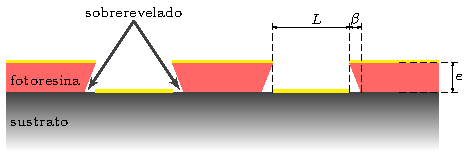
\includegraphics[width=0.75\textwidth]{Esquemas/altura-ancho.pdf}
 				\caption[Perfil de fotorresina para el decapado o\textit{ lift-off}]{Esquema de la fotoresina\index{fotoresina} depositada y revelada, donde se muestra relación de espesor respecto del ancho de linea y el espacio para poder diluirla. El esquema muestra en particular un sobrerevelado\index{sobrerevelado} aproximadamente del 20\%, para obtener buenos resultados durante el procesos de\textit{ lift-off}.}
 				\label{fig:undercut}
 				\end{figure}

 		    En la secuencia de imágenes de microscopia\index{microscopía}\index{microscopía}\index{microscopía!óptica} de la figura \ref{fig:revelado} se muestra como evoluciona el revelado con el tiempo y, en particular, se ve en la última imagnen de esta secuencia, el resultado final de la etapa de litografía y como trasfirió el diseño de manera precisa.

 				%Imagnes revelado
 				\begin{figure}[th]
			 	   	    \centering
			 	   	    \begin{subfigure}[t]{0.235\textwidth}
			        	\includegraphics[width=\textwidth]{Imagenes/revelado1.jpg}
			       		\end{subfigure}
			     		\begin{subfigure}[t]{0.235\textwidth}
			     		\includegraphics[width=\textwidth]{Imagenes/revelado2.jpg}
			    		\end{subfigure}
			     		\begin{subfigure}[t]{0.235\textwidth}
			         	\includegraphics[width=\textwidth]{Imagenes/revelado3.jpg}
			        	\end{subfigure}
						\begin{subfigure}[t]{0.235\textwidth}
			     		\includegraphics[width=\textwidth]{Imagenes/revelado4.jpg}
			        	\end{subfigure}
			     		\caption[Revelado en función del tiempo]{Tiempos crecientes de revelado (de izquierda  a derecha (\SI{2.5}{min},\SI{3.5}{min},\SI{4.5}{min} y \SI{6}{min}) donde se aprecia como se disuelve la resina en la solución reveladora, el cambio de color a medida que cambia el espesor y por último la oblea\index{oblea} revelada por completo. Se deja un 20\% mas del tiempo necesario, para asegurarse un revelado total y para crear el perfil negativo de las paredes, especialmente útil para el proceso de\textit{ lift-off}.}
			     		\label{fig:revelado}\index{lift@\textit{lift-off}}
			     	   	\end{figure}

 		 Se llevó a cabo una segunda etapa de litografía (luego del deposito de Ti\index{titanio}\textbar Au\index{oro} de para los electrodos) para colocar una resina fotocurable, epoxi\index{epoxi}, de alta viscosidad que genera estructuras de hasta \SI{100}{\um} de altura. En la fotografía de la figura \ref{fig:su8} se puede apreciar la alta viscosidad de la misma al momento de hacer el deposito por \textit{spincoating}. Nuevamente los datos para trabajarla se obtuvieron de la hoja de datos del fabricante\cite{Su8,Microchemicals2014} y los detalles experimentales fueron expuestos en  sección \ref{sec:fotolito}, pág. \pageref{sec:fotolito}. Esta resina se uso para hacer la celda electroquímica\index{electroquimico}}, la cual puede contener un volemen aproximado \SI{2}{\ul} de solución. En las microscopia\index{microscopía}\index{microscopía}s de la figura \ref{fig:resultados-su8} se muestra el resultado obtenido luego de alinear y depositar esta resina epoxi\index{epoxi}.

 				%Figura SU8 + alineacion + microscopia\index{microscopía}\index{microscopía} die con Su8
 				%Figura esquema undercutting
 				\begin{figure}[ht!]
 				\centering
 				\includegraphics[width=0.8\textwidth]{Imagenes/SU8.jpg}
 				\caption[Deposito de la resina epoxi\index{epoxi} SU8]{Deposito por \textit{spin-coating }de la resina expoxi para encapsular. Se destaca la alta viscosidad de la misma, lo que permite formar paredes de hasta \SI{100}{\um} de espesor.}
 				\label{fig:su8}\index{spin@\textit{spin-coating}}
 				\end{figure}

 				%Figura esquema undercutting
 				\begin{figure}[th]
			 	   	    \centering
			 	   	    \begin{subfigure}[t]{0.495\textwidth}
			        	\includegraphics[width=\textwidth]{Imagenes/alineacionSU8.pdf}
			       		\caption{Alineación de la segunda máscara\index{máscara} con la pelicula de Ti\index{titanio}\textbar Au\index{oro} ya depositada.}
			         	\label{fig:alineacion}
			     		\end{subfigure}
			     		\begin{subfigure}[t]{0.495\textwidth}
			     		\includegraphics[width=\textwidth]{Imagenes/DIE-SU8.pdf}
			    		\caption{Microscopía de uno de los sensores\index{sensor} con la celda integrada.}
			     		\label{fig:die-su8}	
						\end{subfigure}
						\caption[Alineación y celda integrada en SU8]{Resultados de la alienación de la capa de los electrodos con la máscara\index{máscara} para transferir la fotoresina\index{fotoresina} epoxi\index{epoxi}.}
			     		\label{fig:resultados-su8}
			     	   	\end{figure}

 		\subsection{Películas delgadas de Ti\index{titanio}\textbar Au}

		 Como ya se mencionó anteriormente, los electrodos de los sensores\index{sensor} son de Au\index{oro} y fueron depositados por la técnica de pulverización catódica\index{pulverización catódica} o mas comúnmente conocida por su nombre en inglés \textit{sputtering}\index{sputtering@\textit{sputtering}}. La fabricación consistió primero en depositar una capa de al menos de \SI{20}{\nm} de espesor, llamada capa de  adherencia, la misma puede ser indistintamente de Ti\index{titanio} o Cr\index{cromo}, la cual promueve la adherencia\index{adherencia} del Au; sin esta capa el Au\index{oro} no adhiere sobre superficie\index{superficie}s no metálicas.\cite{Hieber1976} Una vez depositada la capa adherente y sin romper el vacío de la cámara del equipo, se depositó por lo menos \SI{150}{nm} de Au, para lograr un electrodo mecánicamente robusto y con buenas propiedades de conducción eléctrica. Para cada caso, en condiciones constantes, se puede realizar una curva de calibración. La misma se consigue graficando el espesor de las películas depositadas en función del tiempo, con el objetivo de establecer la tasa de depósito\index{depósito} y así poder controlar el espesor de la película. 

				%Grafico de la curva de calibración para el Au
					   		\begin{figure}[ht!]
					   		\begin{center}
							\includegraphics[width=0.75\textwidth]{Graficos/Espesor_Au.pdf}
							\caption[Curca de calibrado para el espesor de los electrodos]{Curva de calibración para establecer la tasa de de deposito de la capa de Au. La misma se realizó por pulverización catódica\index{pulverización catódica} en las condiciones experimentales detalladas en la tabla \ref{tabla:sputt1}.}
							\label{fig:calibracionAu}
							\end{center}
							\end{figure}

		 Se optimizaron las condiciones de \textit{sputtering}\index{sputtering@\textit{sputtering}} para obtener películas homogéneas tanto en espesor como superficialmente. Para lograrlo se variaron los parámetros relevante de la técnica, que son: la aceleración de los iones, determinada por diferencia de tensión entre el cátodo\index{cátodo} y ánodo\index{anodo @ ánodo}; la densidad de corriente y el flujo de Ar\index{argón}. Una vez establecidas dichas condiciones se mantuvieron constante a lo largo de la tesis y se regulo el espesor de las películas controlando el tiempo de depósito, ya que, como estudiaron Peter Sigmund\cite{sigmund1968} y M.P. Seah\cite{Seah2005}, el espesor es directamente proporcional al tiempo según:

	 			\begin{equation}
	 				d=\left(\frac{JYr^3}{e_o}\right)t
	 			\end{equation}


		 Las condiciones de depósito\index{depósito} de cada una de las sucesivas capas se detallan en la tabla \ref{tabla:sputt1}, pág. \pageref{tabla:sputt1}, para las películas metálicas y en la tabla  \ref{tabla:sputt2}, pág. \pageref{tabla:sputt2} para el SiO$_2$. 

		 Para establecer las tasas de depósitos de cada una de la películas depositadas, se midió el espesor por diferentes técnicas. Para monocapas de Au\index{oro} y espesores pequeños típicamente menores a los $30nm$, se utilizó elipsometría ambiental (EA), los detalles experimentales y la base de la técnica ya fueron discutidos en la sección \ref{sec:elipso}, pág. \pageref{sec:elipso}. Para evaluar el apilamiento de sucesivas capas, inspeccionar la homogeneidad tanto en espesor como superficial, se utilizó microscopia\index{microscopía} electrónica\index{microscopía!electrónica} de barrido (SEM) y haz focalizado de iones (FIB), técnica que permite hacer los cortes e inspecciones de secciones transversales de los depósitos en distintos puntos. 

		 			%figuraFIB\index{FIB} de los electrodos
						  \begin{figure}[ht!]
						  \begin{center}
						  \includegraphics[width=0.75\textwidth]{Imagenes/Perfil.jpg}
						  \caption[Sección trasversal de los eletrodos]{Corte transversal de los electrodos, donde se observan detalles de la bicapa Cr\index{cromo}-Au depositada sobre una oblea\index{oblea} de silicio\index{silicio} con un deposito aislante de $SiO_2$.}
						  \label{fig:FIB_electrodos}
						  \end{center}
						  \end{figure} 		
					
	 
		 En la figura \ref{fig:FIB_electrodos} se puede ver un corte transversal de los electrodos, realizado porFIB\index{FIB}, donde se ven los espesores de ambas películas metálicas (Ti, capa adherente y Au), así como la capa dieléctrica de $SiO_2$. También se aprecia la buena homogeneidad en el espesor de cada una de las capas y en la superficie\index{superficie} de la capa de Au, donde ocurrirá finalmente el intercambio electrónico entre las especies redox. Midiendo los espesores de las capas depositadas a distintos tiempos, podemos establecer la tasa de deposito, sacada de la pendiente del figura \ref{fig:calibracionAu}. Como se verá mas adelante, a lo largo del este trabajo, es de suma importancia conocer y controlar los espesores de cada una de las capas.
						
  		\subsection{Decapado de la fotoresina\index{fotoresina} o\textit{ lift-off}}

		 %En algun lugar se puede decir que se elijio lift-off en lugar de etching porque es mejor porque no se coloca fottoresina sobre los electrodos, etc, etc.

		 La última etapa de la fabricación de los electrodos, el decapado de la fotoresina\index{fotoresina}, se conoce mas comúnmente con el nombre en inglés, \textit{lift-off}\index{lift@\textit{lift-off}} y consiste en disolver la fotoresina\index{fotoresina} que quedó de capa de sacrificio. En la figura \ref{fig:undercut} se pueden ver los sitios por donde da comienzo la disolución La misma es completamente soluble en acetona. Cabe destacar, nuevamente, que es importante la disontinuidad de la película de oro\index{oro} para que tenga éxito esta etapa, ya que, si existe continuidad entre la parte que se quiere dejar y la que no, en general provoca imperfecciones en los bordes, o genera que se despegue el metal. Para ello es muy importante saber bien los espesores que se logran durante el deposito, tanto de fotoresina\index{fotoresina} como de película de Au, para regular la distancia que quede entre el metal en el sustrato\index{sustrato} y el metal sobre la resina; el esquema de la figura \ref{fig:undercut} ejemplifica bien esta situación.

					  %Oblea Terminada V1
					  \begin{figure}[ht!]
					  \begin{center}
					  \includegraphics[width=0.75\textwidth]{Imagenes/lift-off.jpg}
					  \caption[Proceso de decapado o\textit{ lift-off}]{Proceso de decapado o\textit{ lift-off}. Fotografía donde se muestra como a medida que se disuelve la fotoresina\index{fotoresina} se va levantando el metal que esta sobre ella.}
					  \label{fig:ultrasonido}\index{lift@\textit{lift-off}}
					  \end{center}
					  \end{figure}

		 Por último, es importarte saber que es necesario aplicar ultrasonido; no alcanza con una simple inmersión de la oblea\index{oblea} en solvente, hay que mantener una constante convexión para la remoción de la fotoresina\index{fotoresina}, que esta debajo del metal. A su vez, este porceso, evita la redepositación del mismo sobre los electrodos (figura \ref{fig:ultrasonido}), ya que si ocurre este fenómeno es muy difícil, una vez que se seca la oblea, remover el metal de desperdicio pegado a los electrodos. Es en esta etapa final del proceso donde se demuestra que si fueron efectivas las etapas de limpieza y revelado. De haber quedado algún residuo durante la limpieza del sustrato\index{sustrato} o haber efectuado un revelado incompleto, llevará indefectiblemente a un desprendimiento de los electrodos del sustrato.

		 Finalmente, en las figuras \ref{fig:ObleaV1} y \ref{fig:ObleaV2}, se muestra el resultado final de la fabricación de los electrodos realizados en obleas de cuatro pulgadas (\SI{10}{\cm} de diámetro) para los dos diseños.

					  %Oblea Terminada V1
					  \begin{figure}[ht!]
					  \begin{center}
					  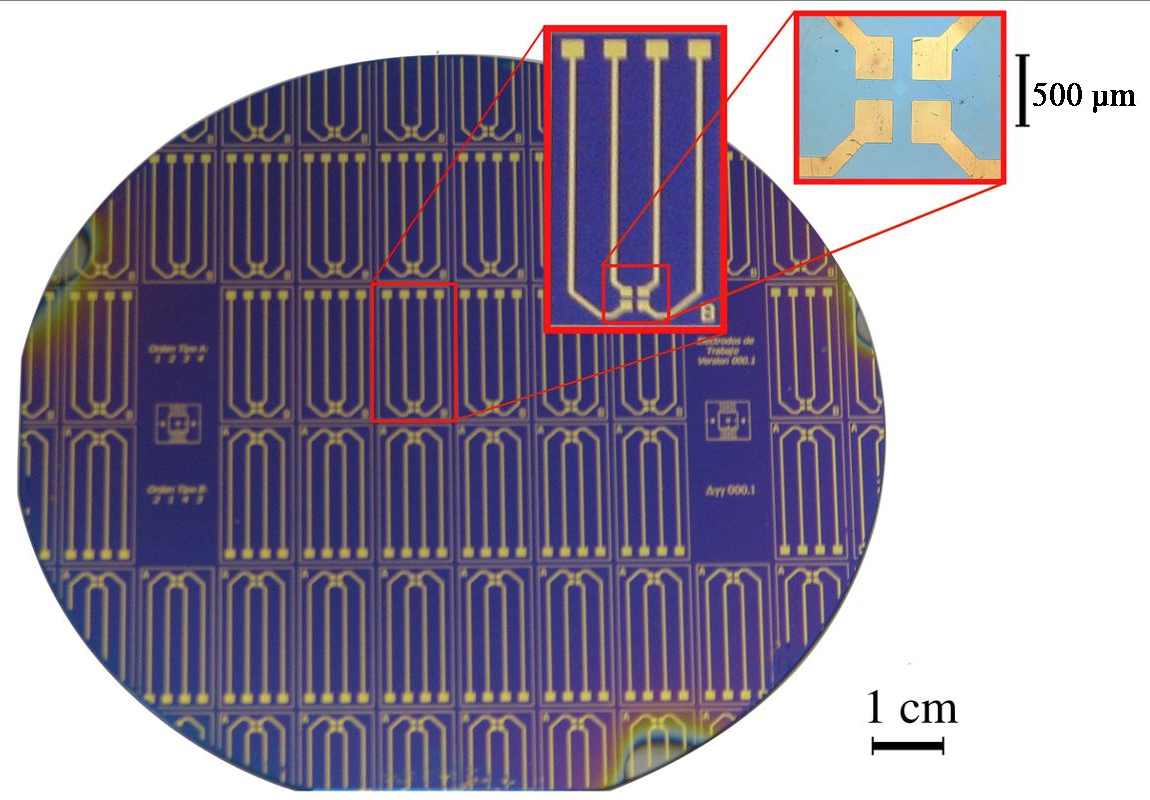
\includegraphics[width=0.75\textwidth]{Imagenes/ObleaV1.jpg}
					  \caption[Electrodos, primera versión]{Primer diseño de los sensores. Oblea de silicio\index{silicio} de \SI{10}{cm} terminada con los 32 sensores.}
					  \label{fig:ObleaV1}
					  \end{center}
					  \end{figure} 	

					  %Oblea Terminada V2
					  \begin{figure}[ht!]
					  \begin{center}
					  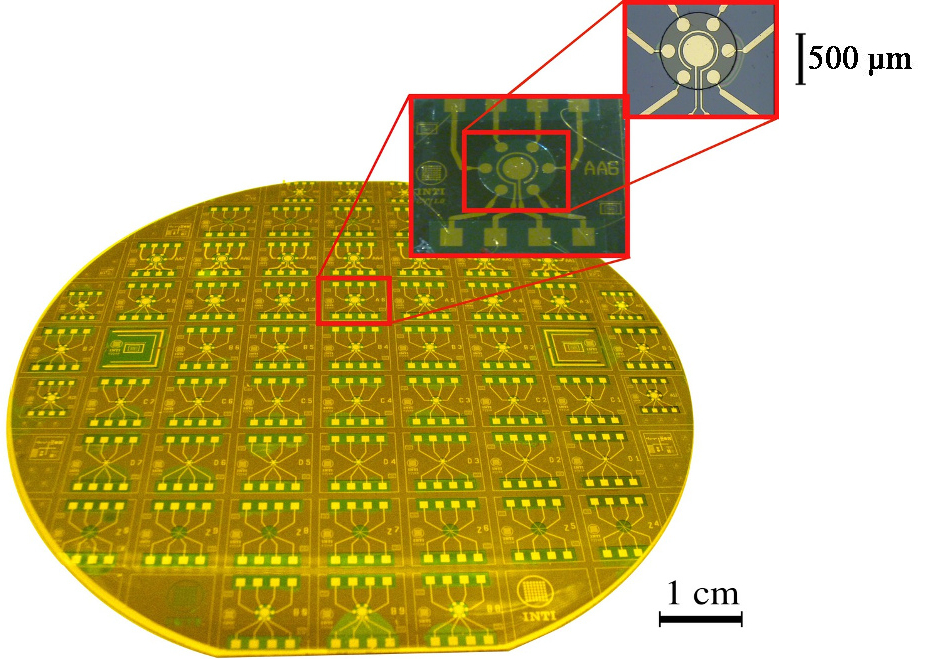
\includegraphics[width=0.75\textwidth]{Imagenes/ObleaV2.jpg}
					  \caption[Electrodos, segunda versión]{Segundo diseño de los sensores. Oblea de silicio\index{silicio} de \SI{10}{cm} terminada con los 46 sensores\index{sensor} que ahora 6 electrodos de trabajo\index{electrodo!de trabajo} cada uno, contraelectrodo\index{electrodo!contraelectrodo} y pseudoreferencia\index{pseudoreferencia}. También se muestra la celda depositada con resina epoxi\index{epoxi} SU-8.}
					  \label{fig:ObleaV2}
					  \end{center}
					  \end{figure} 	
		
\section{Caracterizaciones de los electrodos}

		Se dará cuanta en esta sección de las diferentes caracterizaciones y ensayos practicados sobre los electrodos de Au\index{electrodo!de Au}; básicamente de la respuesta electroquímica\index{electroquimico}, ya que la base de los sensores\index{sensor} son las reacciones de oxido reducción. Es por ello que es fundamental obtener electrodos de respuesta reproducible, confiable y fabricados por un proceso repetible y escalable. 

	\subsection{Respuesta electroquímica\index{electroquimico}}
			 		
		Una vez que los resultados de la fabricación de los sensores\index{sensor} fueron óptimos se evaluó el desempeño electroquímico\index{electroquimico} de los mismos. En el capítulo \ref{chap:Materiales} se describe con detalle el montaje experimental para obtener las voltametría\index{voltametría}s cíclica (VC). Se usaron como sonda\index{sonda}s electroquímica\index{electroquimico}s\index{electroquimico} ferro y ferricianuro de potasio\index{ferricianuro de potasio} (\Ferro\space y \Ferri, \fe), cloruro de hexaaminorutenio(III) (\aminorutenioCompleto, \ru), hidroquinona\index{hidroquinona} (\hidroquinona, \hq) y ferroceno metanol\index{ferroceno metanol} \linebreak (\ferroceno, \fc). La elección de estas sonda\index{sonda}s modelos tiene que ver fundamentalmente con la carga neta de cada una de ellas, y con la reversibildiad de los pares redox. Analizaremos ahora como fue la respuesta de las películas delgadas de Au\index{oro} para cada una de estas sonda\index{sonda}s.
				
		\subsubsection*{Respuesta de ferro/ferricianuro de potasio}	 
			 	
		   En electroquímica\index{electroquimico} este par redox es frecuentemente utilizado para evaluar la calidad de los electrodos, ya que es un par redox cuyas formas oxidada y reducida son económicas, fácil de conseguir, solubles en solución acuosa y se compartan de forma cuasireversible frente al intercambio electrónico electrodo-especie. La reacción que tiene lugar es la siguiente:
			 \begin{equation}
			 \schemestart 
			 Fe(CN)$_6^{4-}$  
			 \arrow{<=>[\scriptsize oxidación][\scriptsize reducción]}[0,1.5] 
			 Fe(CN)$_6^{3-}+e^-$ \schemestop
			 \end{equation}
		  
		  Se graficaron diferentes concentraciones de la sonda\index{sonda} (figuras \ref{fig:Fe_a} y  \ref{fig:Fe_b}) a distintas velocidades de barrido (figuras \ref{fig:Fe_c} y  \ref{fig:Fe_d}) para comprobar la respuestas de los electrodos, la cual se espera que siga el comportamiento descrito por Randle-Sevcik, donde  la intensidad de pico ($i_p$) es proporcional a la concentración ($C$) y a la velocidad de barrido\index{velocidad!de barrido} a la $1/2$ $(v^{1/2})$.
		  
		 	\begin{equation}
			i_p=0.4463nFAC\left(\frac{nFvD}{RT}\right)^{1/2}
			\end{equation}
		
		  Con estos mediciones demostramos a su vez, que el sistema responde a un proceso de difusión\index{difusión} lineal semiinfinita, lo cual era lo que se esperaba para un sistema simple en el que el electrodo esta embebido en la solución soporte {(\SI{0,1}{\milli\Molar} KCl, pH\index{pH}=$5.5$) con la sonda\index{sonda} electroquímica\index{electroquimico}.

			\begin{figure}[ht]
	 	    	\begin{subfigure}[t]{0.5\textwidth}
	         	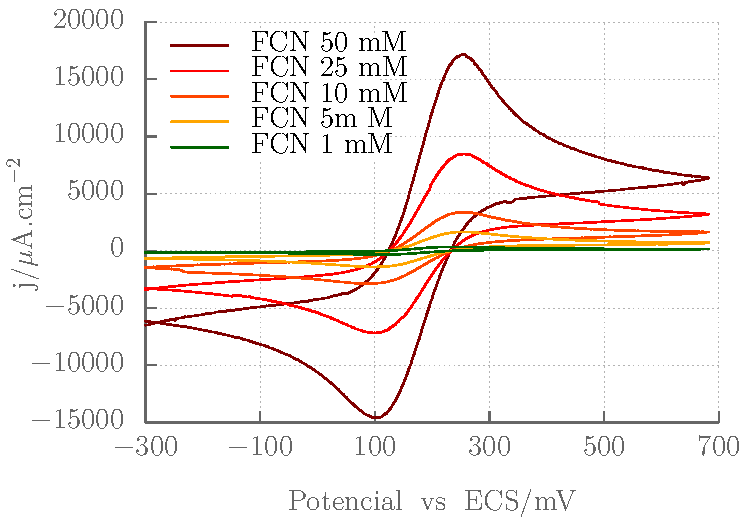
\includegraphics[width=\textwidth]{Graficos/Concentraciones_Fe.pdf}
	        	\caption{Voltametrías cíclicas para la cupla \fe\space a diferentes concentraciones, \SI{1}{\milli\Molar}, \SI{5}{\milli\Molar}, \SI{10}{\milli\Molar}, \SI{25}{\milli\Molar}, \SI{50}{\milli\Molar}. Todas medidas fueron tomadas a \SI{50}{\milli\volt\per\second}.}
	         	\label{fig:Fe_a}
	     		\end{subfigure}
     		 \begin{subfigure}[t]{0.495\textwidth}
	        	\includegraphics[width=\textwidth]{Graficos/Calibracion_Fe.pdf}
	       		\caption{Curva de calibración para distintas concetraciones de la cupla \fe\space valores tomados de la figura \ref{fig:Fe_a}.}
	         	\label{fig:Fe_b}
	     		\end{subfigure}
	     		%\vspace*{0.5cm}

 	     	\begin{subfigure}[t]{0.495\textwidth}
         		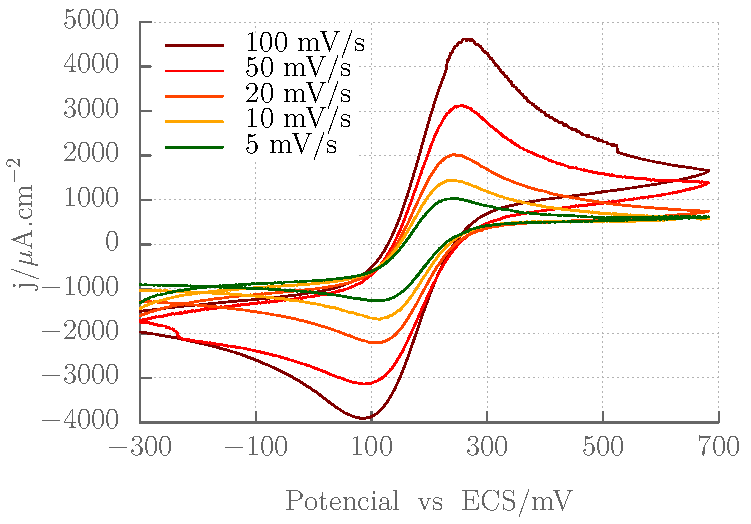
\includegraphics[width=\textwidth]{Graficos/Velocidades_Fe.pdf}
        	    \caption{Voltametrías cíclicas de una solución \SI{10}{\milli\Molar} de la cupla equimolar \fe\space a diferentes velocidades de barrido, \SI{5}{\milli\volt\per\second}, \SI{10}{\milli\volt\per\second}, \SI{20}{\milli\volt\per\second}, \SI{50}{\milli\volt\per\second} y \SI{100}{\milli\volt\per\second}.}
        	    \label{fig:Fe_c}
     		 	\end{subfigure}
     	 	\begin{subfigure}[t]{0.495\textwidth}
        		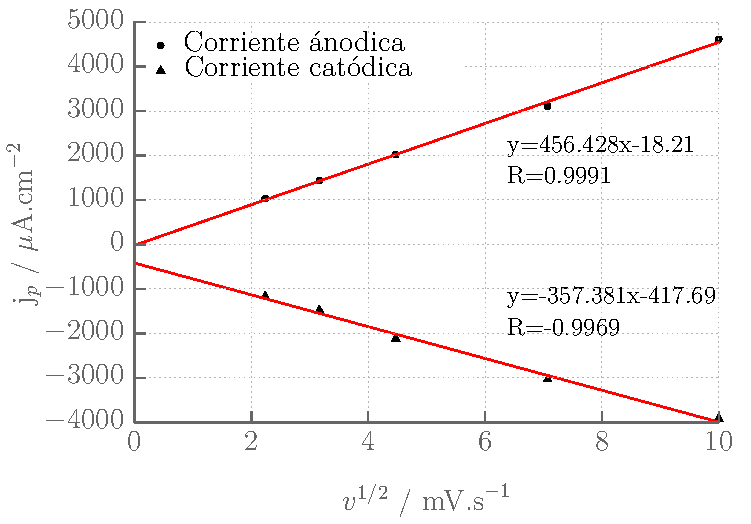
\includegraphics[width=\textwidth]{Graficos/VelocidadesCal_Fe.pdf}
       			\caption[Respuesta a diferentes velocidades de barrido para \fe]{Respuesta frente a diferentes velocidades de barrido para una solución de \fe\space equimolar \SI{10}{\milli\Molar}, se ve una dependencia lineal con la velocidad a la potencia $1/2$.}
         		\label{fig:Fe_d}
     			\end{subfigure}
     		 \caption[Respuesta electroquímica\index{electroquimico} para \fe]{a) Respuesta electroquímica\index{electroquimico} de la cupla equimolar \fe\space para distintas concetraciones, b) curva de calibrado para dichas concentraciones. c) dependencia de la intensidad con la velocidad de barrido\index{velocidad!de barrido} y, d) se observa la dependencia lineal con la inversa de la raíz cuadrada de la velocidad de barrido\index{velocidad!de barrido}. Todos los voltagramas fueron tomadas con un contraelectrodo\index{electrodo!contraelectrodo} de Pt\index{platino} y en una solución 0,1M de NaCl como electrolito soporte.}
     		 \label{fig:ferro-ferri-CV}
     		 \end{figure}
		
			\pagebreak	

	 	\subsubsection*{Respuesta del cloruro de hexaaminorutenio(III)}
	 	  Otra sonda\index{sonda} electroquímica\index{electroquimico}, como veremos mas adelante, de suma importancia en este trabajo, es el cloruro de hexaaminorutenio(III). Esta molécula en solución se disocia para formar el complejo \aminorutenio. La reacción redox que tiene lugar es la siguiente:
	 		 	 	  		\begin{equation}
	 		 	 	 			\schemestart 
					 			 Ru(NH\index{amoniaco}$_3$)$_6^{2+}$  
					 			 \arrow{<=>[\scriptsize oxidación][\scriptsize reducción]}[0,1.5] 
					 		 	 Ru(NH\index{amoniaco}$_3$)$_6^{3+}+e^-$ \schemestop 
	 		 	 	 		\end{equation}
	 	  El intercambio entre los estados de oxidación Ru$^{3+}$/Ru$^{2+}$, responde a un proceso electroquímico\index{electroquimico} reversible, en el cual podemos fácilmente reducir u oxidar el complejo variando el potencial del electrodo de trabajo\index{electrodo!de trabajo}. Habiendo ya comprobado, con el \fe, el buen desempeño de los electrodos respecto de la velocidad de barrido\index{velocidad!de barrido}, se eligió \SI{50}{\milli\volt\per\second} (de uso frecuente para este tipo de mediciones) para las voltametría\index{voltametría}s y se graficaron varias concentraciones de la sonda\index{sonda}, con el objetivo de la curva de calibración correspondiente para \aminorutenio.
			 \begin{figure}[ht]
	 	     \begin{subfigure}[t]{0.495\textwidth}
	         	\includegraphics[width=\textwidth]{Graficos/Concentraciones_Ru.pdf}
	        	\caption{Voltametrías cíclicas para \ru\space a diferentes concentraciones, \SI{6.3}{\milli\Molar}, \SI{3.15}{\milli\Molar}, \SI{1.575}{\milli\Molar}, \SI{0.63}{\milli\Molar}, \SI{0.315}{\milli\Molar}.}
	         	\label{fig:Ru_a}
	     		\end{subfigure}
     		 \begin{subfigure}[t]{0.495\textwidth}
	        	\includegraphics[width=\textwidth]{Graficos/Calibracion_Ru.pdf}
	       		\caption{Curva de calibración para la especie \ru. Los valores fueron tomados de la figura \ref{fig:Ru_a}.}
	         	\label{fig:Ru_b}
	     		\end{subfigure}
	     		\label{rutenio}
	     		\caption[Respuesta electroquímica\index{electroquimico} para \ru]{a) Voltametrías cíclicas para soluciones de \ru\space de distinta concetración y, b) curva de calibración para dichas concentraciones. Todos los voltagramas fueron tomadas a \SI{50}{\milli\volt\per\second} con contraelectrodo\index{electrodo!contraelectrodo} de Pt\index{platino} y en una solución \SI{0.1}{\milli\Molar} de NaCl como electrolito soporte.}
	     	 \end{figure}
			 		 	 
		\subsubsection*{Respuesta del ferroceno metanol}
 	 	  El \fc\space fue otra de las sonda\index{sonda}s electroquímica\index{electroquimico}s\index{electroquimico} que se utilizó. La forma reducida de esta molecular no tiene carga neta, sin embargo su forma oxidada es positiva. La reacción de oxidación/reducción es la siguiente:
 	 	 			%Ecuación redox para el Ferroceno
 	 				 \begin{equation}
 	 	 				\begin{aligned}
 	 	 				\includegraphics[scale=0.65]{Esquemas/Redox-Fc.pdf}
 	 	 				\end{aligned}
 	 	 			 \end{equation}
 	 	  se eligió esta sonda\index{sonda} fundamentalmente por la reversibilidad del par redox, y por la carga neutra de la forma reducida. La \ref{Fig:Fc}muestra la respuesta electroquimica sobre un electrodo de Au\index{electrodo!de Au}, a diferentes concentraciones.
 	 				%Graficos para el Ferroceno
		 		 \begin{figure}[ht]
		 	      \begin{subfigure}[t]{0.495\textwidth}
		          	\includegraphics[width=\textwidth]{Graficos/Concentraciones_Fc.pdf}
		         	\caption{Voltametrías cíclicas para \fc\space a diferentes concentraciones, \SI{1}{\milli\Molar}, \SI{5}{\milli\Molar} y \SI{10}{\milli\Molar}.}
		          	\label{fig:Fc_a}
		      		\end{subfigure}
		      	 \begin{subfigure}[t]{0.495\textwidth}
		          	\includegraphics[width=\textwidth]{Graficos/Calibracion_Fc.pdf}
		         	\caption{Curva de calibración para la especie \fc. Los valores fueron tomados de la figura \ref{fig:Fc_a}.}
		          	\label{fig:Fc_b}
		      		\end{subfigure}
		      	 \caption[Respuesta electroquímica\index{electroquimico} para \fc]{a) Voltametrías cíclicas para soluciones de \fc\space de distinta concetración y, b) curva de calibración para dichas concentraciones. Todos los voltagramas fueron tomadas a \SI{50}{\milli\volt\per\second} con contraelectrodo\index{electrodo!contraelectrodo} de Pt\index{platino} y en una solución \SI{0.1}{\Molar} de NaCl como electrolito soporte.}
		      	 \label{Fig:Fc}
	      		 \end{figure}

		\subsubsection*{Respuesta de la hidroquinona}
		 	 
		 	 	 La \hq\space a diferencia de las otras sonda\index{sonda}s que se utilizó durante la tesis, tiene dos características diferenciales; una es que tanto la forma oxidada como reducida no tienen carga neta (a lo largo de la tesis se desarrollará el concepto de sonda\index{sonda} modelo cargada/neutra para demostrar la permeoselectividad de las membranas),  y la otra es que es el proceso de oxidación de la hidroquinona\index{hidroquinona} en benzoquinona, y su proceso inverso, de reducción nuevamente a hidroquinona, ambos son irreversibles. 

		 	 	 La reacción redox que tiene lugar es la siguiente:
		 	 
		 	 	  			%Ecuacion redox de la HQ
		 	 	 				\begin{equation}
		 	 	 				\begin{aligned}
		 	 	 				\includegraphics[scale=0.75]{Esquemas/Redox-HQ.pdf}
		 	 	 				\end{aligned}
		 	 	 				\end{equation}
		 	 	 			%Graficos para la HQ
				 			\begin{figure}[ht]
				 	     \begin{subfigure}[t]{0.495\textwidth}
				         	\includegraphics[width=\textwidth]{Graficos/Concentraciones_HQ.pdf}
				        	\caption{Voltametrías cíclicas para \hq\space a diferentes concentraciones, \SI{1}{\milli\Molar}, \SI{5}{\milli\Molar} y \SI{10}{\milli\Molar}.}
				         	\label{fig:HQ_a}
				     		\end{subfigure}
			     		 \begin{subfigure}[t]{0.495\textwidth}
				        	\includegraphics[width=\textwidth]{Graficos/Calibracion_HQ.pdf}
				       		\caption{Curva de calibración para la especie \hq. Los valores fueron tomados de la figura \ref{fig:HQ_a}.}
				         	\label{fig:HQ_b}
				     		\end{subfigure}
				     	 \caption[Respuesta electroquímica\index{electroquimico} para \hq]{a) Voltametrías cíclicas para soluciones de \hq\space de distinta concetracionen y, b) curva de calibración para dichas concentraciones. Todos los voltagramas fueron tomadas a \SI{50}{\milli\volt\per\second} con contraelectrodo\index{electrodo!contraelectrodo} de Pt\index{platino} y en una solución \SI{0.1}{\Molar} de KCl como electrolito soporte.}
			     		 \label{fig:HQ}
			     		 \end{figure} 
		 
		En la tabla \ref{tabla:sondas} se resumen las características y los resultados de las voltametría\index{voltametría}s cíclicas para cada una de las sonda\index{sonda}s modelos elegidas. Durante todo el desarrollo de la tesis se utilizaron estos resultados con ánimos de comparar las voltametría\index{voltametría}s sobre los electrodos desnudos y sobre los electrodos con la película mesoporosa.
		  %Tabla resultados EQ
		     \begin{table}[ht]
	  		  \caption{Resultados y características de las sonda\index{sonda}s electroactivas utilizadas.}
	  		  \begin{tabular}{lccc}\toprule
			  Sonda 		& \multicolumn{1}{l}{\hspace{.72cm}Carga especie}\hspace{.5cm} & \multicolumn{1}{l}{\hspace{.5cm}Carga especie}\hspace{.5cm} &\multicolumn{1}{l}{$\Delta$E(mV)}\\
			     		    & \multicolumn{1}{l}{\hspace{.5cm}Reducida}      & \multicolumn{1}{l}{\hspace{.5cm}Oxidada}      &    						     \\ \midrule
	    	  \ferroferri	& \multirow{1}{*}{$4-$}  		& $3-$								   &  150 		  					 \\ \midrule
	  		  \aminorutenio & $2+$							& $3+$								   &  80      						 \\ \midrule
	  		  \raisebox{-.5\height}{\includegraphics[scale=0.4]{Esquemas/Fc.pdf}}   &  0 &     1+      &  103 			                 \\ \midrule
	  		  \raisebox{-.5\height}{\includegraphics[scale=0.4]{Esquemas/HQ.pdf}}	&  0 &     0       &  Irreversible	 				 \\ 
	  		  \bottomrule
	    	  \end{tabular}
	   		  \label{tabla:sondas}
			  \end{table}
		
		\pagebreak			

    \subsection{Incompatibilidad \textit{top-down/bottom-up}}

  		Una vez demostrado el buen desempeño electroquímico\index{electroquimico} de los microelectrodo\index{electrodo!microelectrodo}s, fabricados por técnicas \textit{top-down}\index{top-down@\textit{top-down}}, el siguiente paso fue el deposito de la película mesoporosa\index{película!mesoporosa} sobre los electrodos. Ya se discutió a lo largo de todo el capitulo \ref{chap:Mesoporosos}, las técnicas de deposito y el control sobre la síntesis para obtener películas de diferente porosidad, espesor, adherencia, etc.

  		Nos apoyamos en trabajos similares\cite{Otal2006,Calvo2009b,Fattakhova-Rohlfing2007,Rohlfing2005}, donde utilizan la electroquímica\index{electroquimico} como herramienta para establecer propiedades de las \pdm, pero con la diferencia de que utilizan vidrio\index{vidrio} ITO o vidrio\index{vidrio} FTO como electrodos y desarrollan la electroquímica\index{electroquimico} sobre sistemas más clásicos, no miniaturizados. Sin embargo, una vez depositadas las \pdm\space sobre los electrodos de oro, los resultados no fueron los esperados.  Mostraban, o voltametrias <<planas>>, o curvas donde la respuesta no era clara (figuras \ref{fig:Fe-Au-compa} y \ref{fig:Ru-Au-compa}). 

  		Este problema se encaró de forma sistemática. Partiendo de la hipótesis de que se trataba de algún contaminate, poros bloqueados o defectos durante la síntesis del mesoporosos, se hicieron de nuevo los soles\index{sol} y los ensayos electroquímico\index{electroquimico}s\index{electroquimico} cambiando reactivos, sonda\index{sonda}s, solventes y electrolitos soportes. No pudiendo dar con la solución, se atribuyó el problema a alguna etapa de proceso. Se hicieron muestras control, donde se llevaron en paralelo los procesos de síntesis de películas mesoporosas, (descripto en la sección \ref{sec:cond_y_extr}, pág \pageref{sec:cond_y_extr}) pero sin la película; es decir sometiendo los electrodos a humedad y temperatura de síntesis del óxido. La respuesta electroquímica\index{electroquimico} seguía siendo bastante defectuosa, por lo que se planteó una nueva hipótesis. Esta nueva hipótesis, plantea que el problema radica en someter los electrodos al tratamiento térmico de calcinación\index{calcinación} (\SI{350}{\celsius}).

  		Esta problemática fue central para esta tesis, ya que, surgieron dos vías de acción, 1) Cambiar el material de los electrodos por oro\index{oro} de mayor calidad o platino\index{platino}, 2) sustituir o evitar el paso de calcinación\index{calcinación}. Se consideró la segunda opción mucho mas rica, tanto científica como tecnológicamente, ya que permitía resolver el problema y desarrollar un método de condensación\index{condensación} y extracción\index{extracción} para sintetizar películas delgadas mesoporosas de óxido de silicio\index{silicio!oxido de}. El desarrollo de este método alternativo ya fue extensamente tratado en el capitulo \ref{chap:Optimizacion}.

  		Durante el desarrollo de los métodos alternativos de síntesis de \pdm\space se estudió, en paralelo, como afecta a los electrodos el tratamiento térmico, las resultados de las caracterizaciones se desarrollan a continuación.
			
		\subsubsection{Análisis de la superficie\index{superficie} porXPS\index{XPS}}

			Al surgir el problema luego del tratamiento térmico, se buscó interferencias en la superficie\index{superficie}, ya que trabajos anteriores demostraron difusión\index{difusión} a la superficie\index{superficie} del electrodo de metales provenientes de la capa de adherencia\index{adherencia} \cite{Alonso1990,Moody2003}. Para ello, se analizó con espectroscopia\index{espectroscopia} de fotoelectrones emitidos por rayos (XPS), la superficie\index{superficie} del Au. Se depositaron dos electrodos de Cr\index{cromo}\textbar Au\index{oro} sobre silicio, uno de ellos fue sometido a tratamiento térmico mientras que el otro no. Los resultados se muestran en el gráfico de la figura \ref{fig:XPS}, donde se evidenció la difusión\index{difusión} hacia la superficie\index{superficie}, de cromo\index{cromo} ligado a oxigeno. Esto sugiere que el cromo, utilizado como capa de adherencia, se oxida y difunde cuando los sensores\index{sensor} son sometido a una temperatura de \SI{350}{\celsius}.

				\begin{figure}[ht!]
		 	       	\includegraphics[width=\textwidth]{Graficos/XPS.pdf}
		        	\caption[XPS de peliculas delgadas de Cr\index{cromo}\textbar Au]{Espectroscopia de fotoelectrones emitidos por rayos (XPS) correspondiente a películas delgadas de Cr\index{cromo}\textbar Au\index{oro} con (\usebox{\rojo}) y sin tratamiento térmico  (\usebox{\marron}). Observese los picos correspondiente al cromo\index{cromo} y el aumento de la intensidad relativa del pico correpondiente al oxigeno, indicando la difución de Cr\index{cromo}$_x$O$_y$ hacia la superficie\index{superficie} de los electrodos.}
		         	\label{fig:XPS}
		     		\end{figure}
		
		\subsubsection{Resistencia superficial}

			Una vez demostrada la difusión\index{difusión} a través de las películas de Au, se midió la resistencia superficial, con el objetivo de corroborar algún cambio respecto en las propiedades eléctricas de los electrodos. Se midió la resistencia sobre 3 muestras, una sin tratamientos térmico, otra tratada a \SI{350}{\celsius} y la tercera tratada también a \SI{350}{\celsius} pero en atmósfera de vacío (\SI{1e-5}{\milli\bar}) Los resultados se resumen en la tabla \ref{tabla:resistencia}, donde se corrobora que la resistencia por cuadrado es más alta en las muestras tratadas terminantemente, debido a la difusión\index{difusión} de impurezas hacia la superficie\index{superficie}. 

				\begin{table}[ht!]
			  		  \caption[Resistencia superficial de los electrodos]{Resistencia superficial de Au\index{oro} con y sin tratamiento térmico.} 
			  		  \begin{tabular}{>{\raggedright\arraybackslash}m{3.6cm}>{\raggedright\arraybackslash}m{5cm}} 
			  		  \toprule
					  Muestra & Resistividad superficial $(\Omega/_{\square})$  \\ \midrule
			      	  Au\index{oro} \SI{350}{\celsius} 		  	& $3.720 \pm 0.001$		 \\	  
			      	  Au\index{oro} \SI{350}{\celsius} en vacío	& $3.685 \pm 0.001$		 \\	  
			      	  Au\index{oro} \SI{25}{\celsius}    	  		& $0.595 \pm 0.001$		 \\ 
			      	  \bottomrule
			    	  \end{tabular}
			    	  \label{tabla:resistencia}
			   		  \end{table}
		
		\subsubsection{Voltametrías cíclicas}

			Con el propósito de comparar sustratos, se tuvo la oportunidad de depositar electrodos de oro\index{oro} de mayor pureza, Au4N (99,99\% de \textit{Sigma Al\index{aluminio}drich}) en lugar del Au3N (99,9\% de \textit{Eurometal}). En los gráficos de las figuras \ref{fig:Fe-Au-compa} y \ref{fig:Ru-Au-compa} se tomaron las voltametría\index{voltametría}s cíclicas para las sonda\index{sonda}s \aminorutenio\space  y \ferroferri, sobre electrodos de Au\index{electrodo!de Au} depositados con Au3N calcinado y sin calcinar, con el obejtivo de compararlo con el Au\index{oro} de mayor pureza, Au4N calcinado. 

				\begin{figure}[ht]
		 	      \begin{subfigure}[t]{0.495\textwidth}
		          	\includegraphics[width=\textwidth]{Graficos/Fe-Au-Comparaciones.pdf}
		         	\caption{Voltametrías cíclicas para \fe\space \SI{1}{\milli\Molar} tomadas a \SI{50}{\milli\volt\per\second} en una solución \SI{0.1}{\Molar} de KCl.}
		          	\label{fig:Fe-Au-compa}
		      		\end{subfigure}
		      	 \begin{subfigure}[t]{0.495\textwidth}
		          	\includegraphics[width=\textwidth]{Graficos/Ru-Au-Comparaciones.pdf}
		         	\caption{Voltametrías cíclicas para \ru\space \SI{1}{\milli\Molar} tomadas a \SI{50}{\milli\volt\per\second} en una solución \SI{0.1}{\Molar} de KCl.}
		          	\label{fig:Ru-Au-compa}
		      		\end{subfigure}
		      	 \caption[Comparación entre electrodos calcinados y sin calcinar]{Voltametrías para \fe\space y \ru\space donde se compara la respuesta sobre electrodos de Au\index{electrodo!de Au}4N calcinado (\usebox{\oliva}) con electrodos de Au\index{electrodo!de Au}3N calcinado (\usebox{\negro}) y Au3N sin calcinar (\usebox{\rojo}). Se observa que la respuesta solo es afectada con los electrodos calcinados con Au3N.}
		      	 \label{Fig:Comparacion-Au}
	      		 \end{figure}	

			La primera observación que se desprende de los gráficos es que la respuesta para el Au3N sin tratamiento térmico es prácticamente idéntica a la del Au4N con tratamiento térmico. Por otro lado la respuesta del oro\index{oro} menos purificado, Au3N, sometida a temperatura, muestra una clara irreversibilidad en los procesos de oxido reducción para ambas sonda\index{sonda}s, a tal punto que no se observa la reducción para \ferroferri\space (figura \ref{fig:Fe-Au-compa}, voltametria roja). Con estos resultados y lo expuesto anteriormente, queda claro que la respuesta anómala es debida a una capa superficial, generada por un proceso difusivo durante el tratamiento térmico, la cual dificulta la transferencia electrónica\index{transferencia!electrónica} entre sonda\index{sonda}-electrodo, alejándose de la idealidad, generando una separación de potenciales entre picos anódico y catódica excesivamente grande y voltagramas no reproducibles.
			
		\subsubsection{Microscopía electrónica de barrido}
			  		
			 En las microscopia\index{microscopía} de la figura \ref{fig:Au_compTT} se comparan depósitos de Au\index{oro} tratados térmicamente con no tratados. Se observa un crecimiento en el tamaño de partícula para los tratados térmicamente, a \SI{350}{\celsius}, temperatura para la vía clásica de síntesis de \pdm, lo cual demuestra que esta temperatura es suficiente, para, al menos, producir cambios en el tamaño de los cristales de las películas delgadas de oro, esta transformación también fue reportada a una temperatura de \SI{300}{\celsius} por \v{S}vor\v{c}\'ik\index{Svorcik@\v{S}vor\v{c}\'ik} y colaboradores.}\cite{Svorcik2010}.
			 		\begin{figure}[th]
		 	   	    \begin{subfigure}[t]{0.49\textwidth}
			       	\includegraphics[width=\textwidth]{Imagenes/Au-sinTT.jpg}
			   		\end{subfigure}
			   		\begin{subfigure}[t]{0.49\textwidth}
			   	    \includegraphics[width=\textwidth]{Imagenes/Au-conTT.jpg}
			   		\end{subfigure}
					 \caption[Microscopía comparativa electrodos Au]{Microscopías de barrido electrónico donde se comparan los electrodos sin someter a tratamiento térmico (izquierda) y sometido tratamientos térmico (derecha). Se observa un cambio en el tamaño de las partículas que forman la película.}
					 \label{fig:Au_compTT}	
				     \end{figure}
		 		 		
    \subsection{Comparación entre electrodos}

    	%Compracion AU desnudo, Au\index{oro} INTI\index{INTI} calcinado>

    	Como etapa final de la optimización y caracterización de los sensores, se depositaron \pdm, sobre electrodos de Au\index{electrodo!de Au} de alta pureza calcinado (Au4N), y sobre electrodos de Au\index{electrodo!de Au} de baja pureza (Au3N) realizados a baja temperatura con el método de alto vacio\index{alto@alto vacío} (consultar \ref{sec:trat-vacio}, pág. \pageref{sec:trat-vacio} para más detalle). 

    			 \begin{figure}[ht!]
		 	      \begin{subfigure}[t]{0.495\textwidth}
		          	\includegraphics[width=\textwidth]{Graficos/Ru-F127-CNEA-Calcinado-0-1.pdf}
		         	\caption{Ciclos de VC para \ru\space \SI{0.1}{\milli\Molar} sobre un electrodo de Au\index{electrodo!de Au}4N calcinado, tomadas a \SI{50}{\milli\volt\per\second} en una solución \SI{0.1}{\Molar} de KCl.}
		          	\label{fig:Au4N-Ru1mM}
		      		\end{subfigure}
		      	 \begin{subfigure}[t]{0.495\textwidth}
		          	\includegraphics[width=\textwidth]{Graficos/Ru-F127-INTI-BajaT-0-1.pdf}
		         	\caption{Ciclos de VC para \ru\space \SI{0.1}{\milli\Molar} sobre un electrodo de Au\index{electrodo!de Au}3N sin calcinar, tomadas a \SI{50}{\milli\volt\per\second} en una solución \SI{0.1}{\Molar} de KCl.}
		          	\label{fig:Au3N-Ru1mM}
		      		\end{subfigure}
		      	 \caption[Comparación \pdm\space sobre diferentes electrodos]{Voltametrías cíclicas donde se compara el comportamiento de un electrodo de Cr\index{cromo}\textbar Au\index{oro} de alta pureza sometidos a \SI{350}{\celsius} (a) con otro de baja pureza sin tratamiento térmico ambos recubiertos con una película delga mesoporosa\index{película!mesoporosa} de óxido de silicio\index{silicio!oxido de}\index{silicio} (b).}
		      	 \label{fig:Comparacion-meso}
	      		 \end{figure}
	    
	    Estos experimentos tiene como motivación comparar y validar dos parámetros simultáneamente; por un lado la respuesta de electrodos de Au\index{electrodo!de Au} de alta pureza contra electrodos de Au\index{electrodo!de Au} de baja pureza y, por el otro, el comportamiento de las películas mesoporosas sintetizadas por el método clásico de calcinación\index{calcinación}, con aquellas sintetizadas con el método alternativo de vacío, desarrollado en esta misma tesis y cuyos resultados se expusieron en el capitulo \ref{chap:Optimizacion}.
    	Los resultados fueron satisfactorios, tal como se muestran en las figuras \ref{fig:Au4N-Ru1mM} y \ref{fig:Au3N-Ru1mM}, donde se ve una respuesta prácticamente idéntica tanto para el sistema calcinado como para el sistema de baja temperatura. 
    	Tanto la forma de Las diferencias que se observadas se discutirán en el próximo capitulo ya que tienen que ver con el trasporte y el modelo planteado para las difusión\index{difusión} de sonda\index{sonda}s dentro de las películas porosa y no, con la naturaleza de la película de Cr\index{cromo}\textbar Au.


		   	% En la figura \ref{} se compara la voltametría\index{voltametría}, para \aminorutenio\space sobre un electrodo de Au\index{electrodo!de Au}3N y sobre otro recubierto con mesoporoso. Se ve allí, para el electrodo desnudo, que tanto la intensidad como la separación en potencial entre los picos catódicos y anódicos, muestran un proceso mucho mas irreversible de lo esperado para esta sonda\index{sonda}, indicador de algún problema en la trasferencia electrónica entre analito y electrodo. La respuesta con el mesoporoso depositado es similar, con la diferencia que aquí se muestra como este ingresa en la película, la explicación detallada de este tipo de voltagrama se trata a fondo en el siguiente capítulo. Este resultado fue otro de los indicadores de que la película mesoporosa\index{película!mesoporosa} no es el problema, sino el electrodo.

		% Aca va el cambio de au vs tratamientos de bajas temperaturas y aplicable a nuevos sustratos y por supuesto mucho mas economico (por el Au).

\section{Conclusiones parciales}

	Se revieron, a lo largo de este capítulo, los resultados obtenidos durante el proceso de fabricación de los microelectrodo\index{electrodo!microelectrodo}s de Au. Se hicieron dos diseños, de los cuales el segundo (retroalimentado de la experiencia del primero) es mas compacto, incorpora mas electrodos por sensor\index{sensor} y prevé el uso de contraeletrodo y referencia integrados en el mismo.
	
	Los mismos fueron fabricados por el conjunto de técnicas conocidas como \textit{top-down}\index{top-down@\textit{top-down}}, ftoolitografia, deposición por
	pulverización catódica y \textit{lift-off}\index{lift@\textit{lift-off}}, entre otras. Encontradas las condiciones óptimas de proceso para cada etapa, y, conforme con los resultados, se evaluó la performance electroquímica\index{electroquimico} de los mismos, la cual resulto ser muy satisfactoria. La siguiente etapa fue la de	colocar la \pdm\space sobre ellos, fue en esta etapa donde surgieron algunas dificultades, algunas de ellas discutidas en el capitulo \ref{chap:Mesoporosos}. En particular, en lo referente al sensado electroquímico\index{electroquimico}, pudimos detectar fenómenos de difusión\index{difusión} hacia la superficie\index{superficie} del electrodo, durante la calcinación\index{calcinación} de las películas de SiO$_2$ mesoporosa\index{película!mesoporosa} sobre ellos, impidiendo el intercambio de electrones sonda\index{sonda}-electrodo. 

	Este fue uno de los motores (junto con con otros como utilizar polímeros, evitar calcinaciones, abaratar costos, etc.) para el desarrollo de procesos de síntesis de películas mesoporosas de SiO$_2$, a temperaturas menores que las clásicas de calcinación\index{calcinación}, donde se minimizan los procesos difusivos y no es necesario recurrir a material de ultra pureza.
	
	Para concluir, se fabricaron con electrodos de excelente desempeño electroquimico. Sobre ellos se depositaron películas mesoporosas depositas por los métodos desarrollados en el capitulo \ref{chap:Optimizacion}, y se pudo corroborar la respuesta electroquímica\index{electroquimico} con otros sensores\index{sensor} fabricados con Au\index{oro} de alta pureza con \pdm\space calcinadas, es decir por una vía clásica de síntesis.

	En la figura \ref{fig:flujo-microfab} se resumen las etapas de trabajo para llegar a obtener los sensores, cuyas propiedades de transporte\index{transporte} a través de la estructura de nanoporoso serán evaluadas en el próximo capitulo.
				
				\newpage
				
				\begin{figure}[ht!]
		 	       	\includegraphics[width=\textwidth]{Esquemas/flujo-microfab.pdf}
		        	\caption[Fabricación de sensores, flujo de procesos.]{Diagrama donde se resumen las etapas en la fabricación de los sensores\index{sensor} y los desafíos que surgieron durante las mismas. El cuadro lila es el sistema de sensores\index{sensor} de estudio para los próximos capítulos donde se evaluarán las capacidades como sensores\index{sensor} de dichos sistema.}
		         	\label{fig:flujo-microfab}
		     		\end{figure}


% Una vez obtenida y analizada la respuesta sobre los electrodos de Au\index{electrodo!de Au} desnudo (esto es, sin recubrimiento de la película mesoporosa) se discutirá en los próximos capítulos como varia esta respuesta y como podemos sacar conclusiones acerca del transporte\index{transporte} a travéz de peliculas mesoporosas y también de cuestiones estructurales de las mismas.


% durante la tesis muchas medidas, bla bla y entonces los proximos capitulos es indistinto con un electrodo pleno o con electrodos con diseño transferido sistintas areas, electrodos de ag/cl y de calomel..... pseudoreferencia\index{pseudoreferencia}.... etc. etc  ... Para adoptar un criterio y con animos de poder comparar los resutlados siempre se normalizaron con la densidad de corriente y contra la referencia de calomel.